\chapter{Virtualization and Cloud Computing}
\label{chapter:cloudcomputing}

%General about the shift that has been happening towards virtualized and software applications
\textcolor{red}{More prepping on virtualization}

Virtualization is a technology that allows creating valuable IT services using resources that are traditionally bound to hardware. The term virtualization refers to abstraction of compute resources from applications and end-users consuming the service \cite{Xing2012}. Virtualization allows hardware operators to use the physical machine's full capacity by distributing the computing power to multiple users or environments simultaneously. \cite{RedHat} In the context of telco, virtualization is the main objective to replace the costly dedicated hardware by implementing several centralized control plane functions and other services with distributed solutions. These services and solutions may be allocated on-demand over a pool of dependable, dynamically contracted computing and networking resources that are easy to manage. \cite{Bosch2011} Virtualization brings down the expenses arising from acquiring, updating, and managing the hardware \cite{Lingayat2018}\cite{Toimela2017}.

% Hardware support for GPU, Ethernet card
Virtualization involves the construction of an isomorphism that maps a virtual guest system to a real host. This isomorphism maps the guest state to the host state \cite{Xing2012}. Virtualization abstracts the underlying resources such as CPU, GPU, storage, network, and memory from the application running on the host. Previously the virtualization support was purely software-based, which included latency for the application requiring virtualization. The introduction of x86 virtualization for CPUs by Intel's VT-d and AMD's AMD-V allowed minimal software to be used with virtualization, thus reducing the overhead for CPU operations with direct access.

\section{Virtualization types}

A traditional physical server has applications running directly on the host operating system (OS). The solution limits overhead from extra layers such as hypervisor or virtual machine (VM), but compromises the usage of resource efficiency, security and limits compatibility. Two virtualization technologies, hypervisor-based virtualization and container-based virtualization, have been introduced to improve these features. Hypervisor-based virtualization provides strong isolation of a complete operating system whereas container-based virtualization strives to isolate processes from other processes at little resource costs \cite{Eder2016}. Figure \ref{fig:VirtualizationTypes} describes the stack of these two virtualization types and a traditional physical server.

Hypervisor-based virtualization involves hypervisors to emulate hardware for creating virtual machines and wraps each application instance running is wrapped inside a VM with a dedicated guest OS, binaries, and libraries. Hypervisor allows to fully emulate another computer, therefore it is possible to emulate other types of devices for example a smartphone or a gaming console \cite{Eder2016}. This is useful especially when developing software for mobile platforms allowing testing without the need of target device. The inclusion of an additional layer of hypervisor over host operating system is highly secure solution and compatible with various host operating systems and processor architectures via hardware emulation \cite{Lingayat2018}. However, the added layers depreciate the performance of the virtual machine significantly as the hypervisor directs traffic between physical and virtual hardware. Resources of the server are wasted, especially when multiple VMs are hosted on the same server. %

Recent evolution is a lightweight alternative to the virtual machine called containers. Container-based virtualization got gained popularity when Docker, a tool to create, manage, distribute, and run containers got a lot of attention by combining different technologies to a powerful virtualization software \cite{Eder2016}. Container-based virtualization has proven very efficient regarding performance and orchestration, and many industries have migrate their virtualized environment to run on Linux containers. Containers share parts of the host operating systems kernel as well as the host’s libraries and binaries where appropriate, and isolate each container by encapsulating them with their required services and packages.  These containers can also include application specific binaries and libraries. Linux containers utilize less storage space and consume optimal computational power, giving a improvement in performance in terms of resource overhead, space requirements and speed \cite{Toimela2017}\cite{Lingayat2018}. Containers are highly portable and compatible due to standardized packaging format managed by Open Container Initiative (OCI)\cite{OCI}. Managing of even thousands containers can be easily achieved with container orchestration and scheduling tools such as Kubernetes. Containers are isolated from each other by using various packaging techniques such as cgroups and kernel namespaces, and utilize kernel features to create an isolated environment for processes. In contrast to hypervisor-based virtualization, containers do not get their own virtualized hardware but use the hardware of the host system. Not having to emulate hardware and boot a complete operating system enables containers to start in a few milliseconds and be more efficient than classical virtual machines \cite{Eder2016}. The lack of security features comes with a cost of frail security, thus Chapter \ref{section:security} points out that the security mechanisms of Linux container is partial against more advanced attacks. To improve the security of containerized environments, Chapter \ref{chapter:katacontainers} introduces Kata Containers. This quite recently developed solution combines the security of virtual machine and speed of containers with the help of custom container runtime.

\begin{figure}[ht]
  \begin{center}
    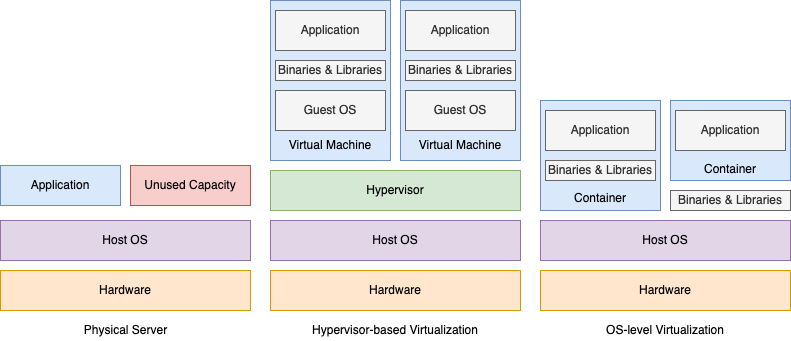
\includegraphics[width=13.5cm]{images/VirtualizationTypes.png}
    \caption{Physical server and two types of virtualization}
    \label{fig:VirtualizationTypes}
  \end{center}
\end{figure}

\section{Cloud computing}

Data centers, with the help of hardware virtualization, offer on-demand availability of computer resources such as computing power or data storage. This pay-per-use offering is described as cloud computing. Cloud computing offers customers the ability to start businesses without having to pay huge upfront capital expenses and the exhibition to scale the IT infrastructure up and down as a business evolves without worrying about over or under provisioning \cite{Xing2012}. It has been a vital enabler in the field of Information Technologies allowing the success of cloud applications such as Google Docs, Slack, and Dropbox. The ubiquitous and connected computing provided allows higher usage of resources and access from anywhere via internet, thus improving performance, reducing costs, and allowing easy access to hosted applications. Public cloud services end-user spending worldwide has been growing steadily and is expected to grow 40\% from 2020's 219 billion euro to 307 billion euro only in two years \cite{PublicCloudStatista}.

The general idea behind cloud computing technology dates back to the emerge of grid computing in early 1990s as an idea for making computing power as easy to access as an electric power grid. This cloud model promotes availability and is composed of five essential characteristics. These characteristics are on-demand self-service, ubiquitous network access through Internet-enabled devices, location independent resource pooling, rapid elasticity, and pay per use. A cloud is a pool of virtualized resources across the internet, that follows pay-per-use model and can be dynamically reconfigured to satisfy the user requests by provisioning virtual machines. Cloud computing is a service model for IT provisioning, often based on virtualization and distributed computing technologies \cite{Lombardi2011}. \cite{Xing2012}

Cloud computing offers four different service models: public, private, hybrid, and community clouds. Cloud is typically a centralized server, such as, Microsoft Azure or Red Hat OpenShift. These cloud platforms provide users with scalable resources, high availability and fast connections. Cloud platforms can be public, such as the before-mentioned ones, or a private cloud serving only selected customers. Private clouds are usually deployed on-premises within a corporate firewall by businesses with requirements for additional control and privacy over the network. Hybrid cloud is a combination of both, made up of on-premises infrastructure, private cloud services, and a public cloud. The hybrid approach brings enterprise with agility to use the best suitable solution for each occasions. \cite{NetApp} Community cloud is a resource pool that consists of an aggregation of several providers, which can be shared by a certain group of users. Although different deployment models of cloud computing cater to different consumers, they all have common characteristics such as massive scale, resilient computing, homogeneity, virtualization, low cost software, geographic distribution, service orientation, and advanced security technologies. \cite{MicrosoftAzure}\cite{Taleb2017}\cite{Xing2012}

% Emerge of various applications with different requirements
% Optimize latency and throughput in network
% Intro to Edge





%Telecommunications computing ... The computing locates in various different sizedata centers as described in Figure \ref{fig:AirFrame}. Central data centers are built to massive warehouses that take advantage of centralized maintenance and 

%Telco environment
%Central data center vs edge cloud in general
%3    - Efficient capacity vs low latency \& efficient transport


\section{Multi-access Edge Computing}

Multi-access Edge Computing (MEC) is an emergent architecture where cloud computing services are extended to the edge of networks leveraging mobile base Radio Access Network (RAN) improving the delivery of content and applications to end-user. As a promising edge technology, it can be applied to mobile, wireless, and wireline scenarios, using software and hardware platforms, located at the network edge in the vicinity of end-users. MEC provides seamless integration of multiple application service providers and vendors toward mobile subscribers, enterprises, and other vertical segments. It is an important component in the 5G architecture which supports variety of innovative applications and services where ultra-low latency is required. \cite{Abbas2018}

Figure \ref{fig:AirFrame} describes the differences in edge and central data centers.  

\begin{figure}[ht]
  \begin{center}
    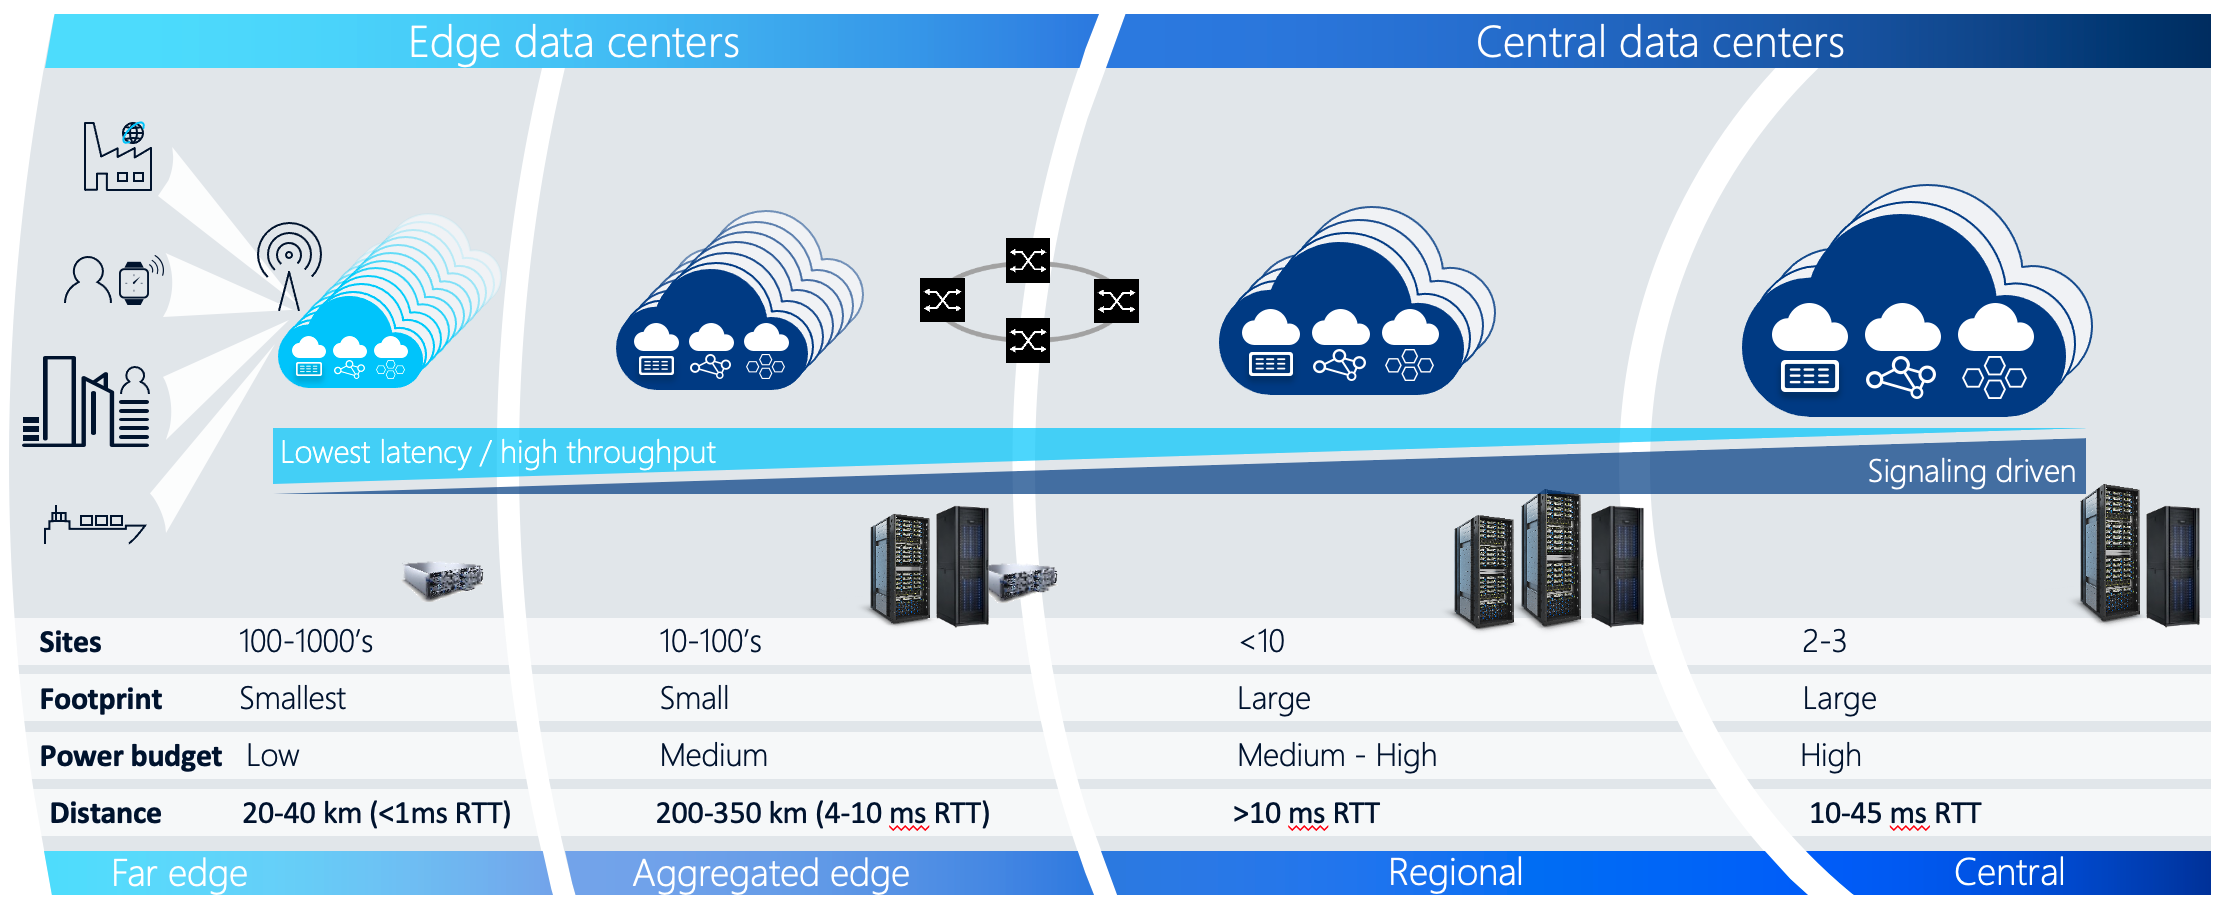
\includegraphics[width=13.5cm]{images/AirFrame.png}
    \caption{Far edge comparison to central data center \cite{AirFrameOpenEdgeServer}}
    \label{fig:AirFrame}
  \end{center}
\end{figure}

MEC improves network efficiency by processing and storing data on the mobile network cell instead of hauling it completely back to regional or central data centers for processing. The data can be processed partially or completely on the MEC node. For example, large public venues, such as stadiums or arenas, are good candidates for MEC, especially where localized venue services are important. In this use case, video created at a sports event or concert is served to on-site consumers from a MEC server, running appropriate applications located on the stadium premises. This video traffic is locally stored, processed and delivered directly to users at the event and does not require backhaul to a centralized core network and to then be returned to the user at the venue. The local processing of data reduces perceived latency on end-user and limits stress on the backhaul network. \cite{Brown2016}

MEC covers two edge entities: aggregated edge and far edge. Aggregated edge locates usually at most 200 to 350 kilometers away from the end user and guarantees 4 to 10 millisecond round trip time (RTT). The RTT is low in comparison to central data center latency, however it is not low enough for mission-critical and real-time applications requiring less than 1 ms latency. For example, self-driving cars and factory robots might require ultra-low latency reply from the applications.

\subsection{Far Edge Cloud}

Far edge cloud locates at most 20 to 40 kilometers away from the end user, and thus is able to offer sub one millisecond RTT, as service level agreement of the 5G network \cite{Parvez2018}. The ultra-low latency is critical for applications requiring instant reply from the server. Offloading tasks, computing, and storage to nearby cloud allows thin clients, such as cellphones or dashboards, with limited resources to support applications with resource heavy requirements, such as applying machine learning models to obtained video feed in real-time. Migration of tasks to resource-rich centralized servers also helps power agnostic user-equipment to save battery life. Far edge cloud setup is minimal in size, footprint, and power budget. It is flexible to install as it can be located in an office or apartment building with no requirement for extensive server chassis. \cite{AirFrameOpenEdgeServer}

Far edge cloud units are highly localized. A network might consist of hundreds or thousands of these units. The data processed does not always travel further away from the end-user enhancing the security and integrity of the data. The localized data schemes help also service providers, as they are not obliged to apply multiple data protection laws, GDPR for example, at the same time. FEC units also handle sensitive, user-related data. Thus, it is crucial to secure the infrastructure from external threats and internal attacks, such as third-party applications hosted on the infrastructure.

\subsection{Applications}
\label{subs:applications}

MEC architecture unlocks potential of new applications, and thus is a new revenue stream for mobile network operators. Some recognized applications harnessing the use of MEC include augmented reality (AR), video analytics, and connected vehicles.

AR enables real environment user experience by combining real and virtual objects existing simultaneously. Recent AR applications have become adaptive in sound and visual components, such as news, TV programs, sports, object recognition, and games. AR applications often demand high computational resources, low latency for reasonable quality-of-experience, and high bandwidth. MEC can empower AR applications by maximizing throughput by offering computational resources nearby the end-user withing low-latency and high throughput channel instead of relying on the core-network. \cite{Abbas2018}

Surveillance cameras traditionally have been streaming data back to the server, which decides how to perform data analysis. Due to the growing number of these cameras, it adds an enormous stress to the network with the constant data streams. In this example, MEC will be beneficial by implementing intelligence to the device by transmitting data only when motion is detected. Also, it can help public safety with detection of traffic jams, accidents or forest fires.

The edge computing technology plays a key role in website performance optimization, such as caching HTML content, reorganizing web layout, and resizing web components. HTTP requests from user pass the edge server which helps with content delivery. The server handles user requests by performing a number of task to load webpages on the user device interface. \cite{Abbas2018}

Connected vehicles are facilitated with cellular connection allowing them to communicate with other users on the road. MEC based road communication system could allow two-way communication between vehicles via road side units. For example, one vehicle could warn another vehicles about upcoming road jam or approaching pedestrians. The road side unit could also warn passing cars about dangerous conditions based on the sensors equipped in it. \cite{Abbas2018}

\section{Security concerns}
\label{section:security}

Integrity and confidentiality concerns are still problems in cloud computing that call for effective and efficient solutions. Cloud nodes are inherently more vulnerable to cyber-attacks and breaches than traditional solutions, given their size and the underlying complexity of services bringing unprecedented exposure to third parties of services and interfaces. \cite{Lombardi2011}

Cloud and Edge Computing security cover the same threats as core computing. However, these platforms are generally not offering the same security-rich features and security policies and procedures. Edge Computing is typically more vulnerable to local introspection attacks. Edge Computing units might be vulnerable to Denial-of-Service attacks, which might drain the resources of the unit thus rendering all hosted services useless. Furthermore, malicious antagonists can misuse virtual resources and not only affect the whole system itself but also the connected devices such as IoT sensors or user equipment. \cite{EdgeComputing5G}\cite{Abbas2018}

Cloud and edge computing allow service providers and MNOs for more flexible and cost-efficient service deployment due to shared and decentralized infrastructure. Especially MNOs seek to unlock extra revenue streams by offering their infrastructure to host applications such as mentioned in Chapter \ref{subs:applications}. In order to mitigate costs from the application, it is resource-efficient to run multiple instances or applications from various parties on a single server. This approach applies to companies who own dedicated servers or cloud computing providers with various data center options. These multi-tenant environments may host applications also from untrusted parties. Regardless of the isolation offered by Docker with cgroups and namespaces, the containers still share the same kernel. This architectural decision might expose applications, as it was noticed in 2019 \cite{CVE-2020-14386}\cite{CVE-2019-5736} when attackers could elevate their access to host root. The escaping of container and horizontal traversal via shared kernel creates a security thread of application data integrity. The virtualization technique domain is buoyant with many competing emerging technologies for hardening containers and VMs, solving the equation of isolation versus overhead. This thesis researches and evaluates Kata Containers (KC) to adding an extra layer of security to avoid the container escapes on host compromise on a shared platform with minimal overhead. \cite{EdgeComputing5G}

\section{Isolation mechanisms}

Sharing kernel of the host operating system exposes applications to potential security threats. Companies handling and hosting sensitive data in cloud computing environments have developed new ways to solve the the trade-off between isolation and speed. Kata Containers is a promising solution which unifies the security advantages of virtual machine with the speed and flexibility of containers. In Kata Containers, each containers is equipped with its lightweight virtual machine and a mini kernel, providing container isolation via hardware virtualization which improves the security layer \cite{Kumar2020}.

Kata Containers is not the sole option providing secure container runtime nor isolation in the container kernel layer. Microsoft offers a container instance isolation option inside Azure with Hyper-V. The hardware isolation is based on VMs, likewise in KC and Firecracker, thus leveraging the additional kernel layer. \cite{Hyper-V}

gVisor provides a second isolation method, differing from Kata Containers and Firecracker. gVisor intercepts application system calls and acts as the guest kernel without translating through virtualized hardware. The architecture can be thought of as a merged kernel and VMM. gVisor includes OCI runtime runsc, which provides the isolation boundary between the application and host kernel. Google develops gVisor, and it is harnessed in various Google's cloud products such as Kubernetes Engine \cite{GKE} and Cloud Run \cite{CloudRun}. \cite{Debab2021}\cite{gVisor}

A second approach for container isolation is IBM Nabla \cite{Nabla}. Nabla containers use library OS, also known as unikernel, to avoid system calls and reduce the attack surface. Nabla is based on a custom VMM named Nabla Tender to manage lightweight VMs executing unikernels. Nabla containers only use seven system calls, blocking all others via a Linux seccomp policy. The Nabla Tender intercepts hypercalls related to storage and network from unikernel VMs and translates them into syscalls to the host. \cite{Debab2021}

All the before-mentioned projects are open source and actively maintained. However, Nabla seems to be slightly less active in comparison to the other projects. Commercial and enterprise cloud platforms, such as AWS, uses Firecracker, and GKE uses gVisor. However, for security reasons it is unknown which approaches are used in the other platforms to isolate containers.



%You can translate your latex file to rtf with the \texttt{latex2rtf} command in the
%kosh.aalto.fi shell server. Then, the line breaks
%will not be problems for the proofreader of Word.

%Note also that if you have a section or a subsection, you have to have
%at least two of them, or otherwise the section or subsection title is
%unnecessary. Same with the paragraphs: you should not have sections
%with only one paragraph, and single sentence paragraph.

%Aalto library has a comprehensive citation guide ~\cite{bibinstructions}.


% Comment: If your sentence ends in a capital letter write \@ before the period

% If you do need a normal space after a period (instead of
% the longer sentence separator), use \  (backslash and space) after the
% period. Like so: a.\ first item, b.\ second item.